\chapter{Requirement Analysis}
\label{chap:requirement-analysis}

\section{Stakeholder Analysis}
\label{section:stakeholder-analysis}
\subsection{Primary Stakeholders}
\label{subsection:primary-stakeholders}

\begin{enumerate}[leftmargin=80pt]
    \item \textbf{Users:} Users represent the target users of our application. They often struggle to find parking, and our app helps by providing parking availability information. For specification of our users see \ref{section:target-user}.
    \item \textbf{Parking Area Owners:} Parking area owners are people or organizations that manage parking facilities around the campus. Due to financial constraints, their options for utilizing the parking area are limited, but they still want to provide availability information for visitors. They play a key role as site owners, controlling the existing infrastructure within the system.
\end{enumerate}

\section{User Stories}
\label{section:user-stories}
<TIP: Write user stories for each of your stakeholders here./>

User stories are a technique used in agile software
development to capture and describe functional requirements from an end
user's perspective. They are a way of expressing software features or
functionality in a simple, non-technical language that can be easily understood
by both developers and stakeholders.

\section{Use Case Diagram}
\label{section:use-case-diagram}
<TIP: Write a use case diagram for your project here. Refer to an
article “What is a use case diagram?” by Lucidchart for help./>

\section{Use Case Model}
\label{section:use-case-model}
A use case is a detailed description of how a system
interacts with an external entity (such as a user or another system) to
accomplish a specific goal. Use cases provide a high-level view of the
functionality of a system and help in capturing and documenting its
requirements from the perspective of end users.

<TIP: Write use cases for your project here. Make sure to use the
appropriate type of use case for each scenario (brief, casual, and fully-dressed
use case)./>

\section{User Interface Design}
\label{section:user-interface-design}
<TIP: Put the initial design of your application here. You can
showcase a detailed design of a specific page or a sitemap of your application.
See an example below./>

\begin{figure}[h]
    \centering
    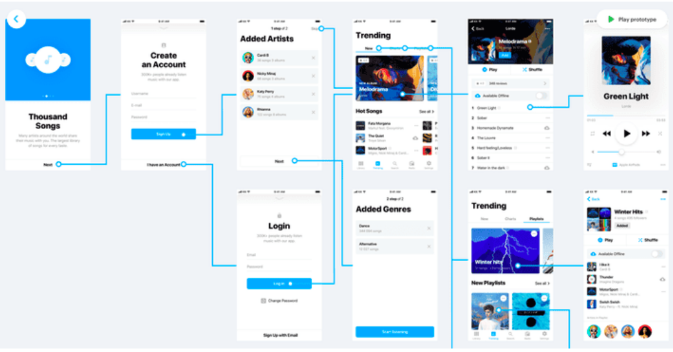
\includegraphics[width=0.8\textwidth]{examples/user-interface-design.png}
    \caption{User Interface Design}
\end{figure}